\section{Substring search}
\subsection{Aim}
To search whether a substring occur in a string

\subsection{Code}
\begin{lstlisting}
DATA SEGMENT
    str DB 'hello world', '$'
    strlen EQU $~str
    nvowels DW ?
DATA ENDS

CODE SEGMENT
ASSUME CS:CODE, DS:DATA
START:
    MOV AX, DATA
    MOV DS, AX
    MOV CX, strlen
    XOR BX, BX
    LEA SI, str

COMP:
    CMP BYTE PTR SI, 'a'
    JE INCR
    CMP BYTE PTR SI, 'e'
    JE INCR
    CMP BYTE PTR SI, 'i'
    JE INCR
    CMP BYTE PTR SI, 'o'
    JE INCR
    CMP BYTE PTR SI, 'u'
    JE INCR
    JMP INCRC
    
INCR:
    INC BX
    
INCRC:
    INC SI
    LOOP COMP
    
EXIT:
    MOV nvowels, BX
    MOV AH, 4CH
    INT 21H
CODE ENDS
END START
\end{lstlisting}

\subsection{Output}
\begin{center}
	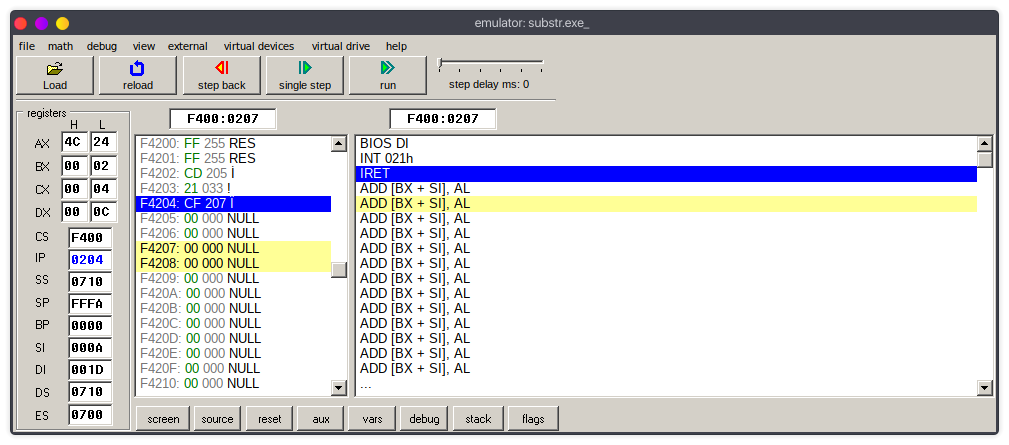
\includegraphics[width=0.90\textwidth]{img/p19/ss1.png}
	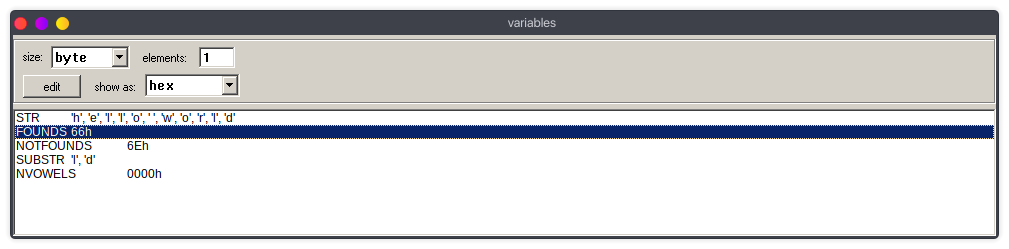
\includegraphics[width=0.90\textwidth]{img/p19/ss2.png}
	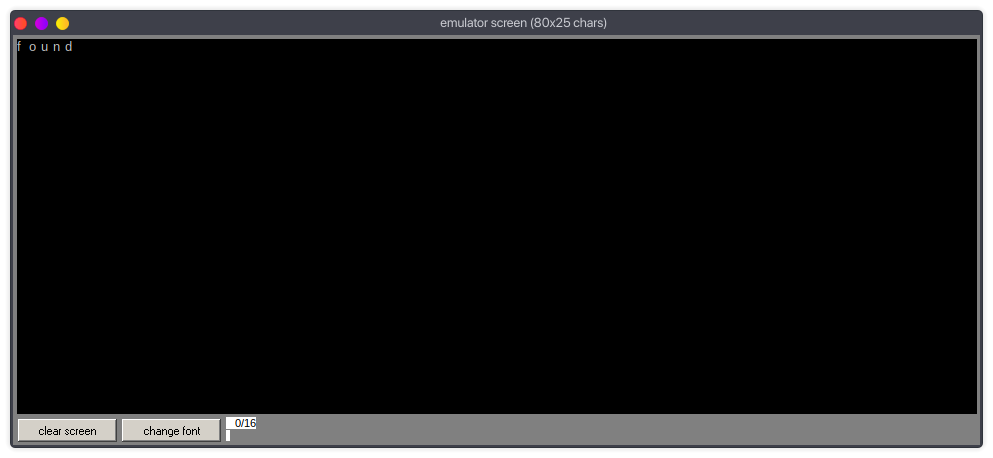
\includegraphics[width=0.90\textwidth]{img/p19/ss3.png} \\
	Output for 'ld'\\
	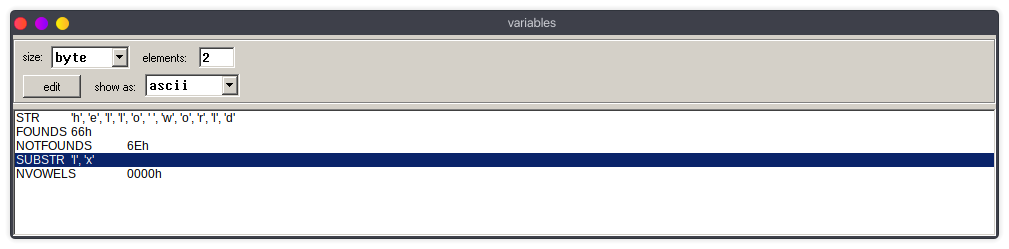
\includegraphics[width=0.90\textwidth]{img/p19/ss4.png}
	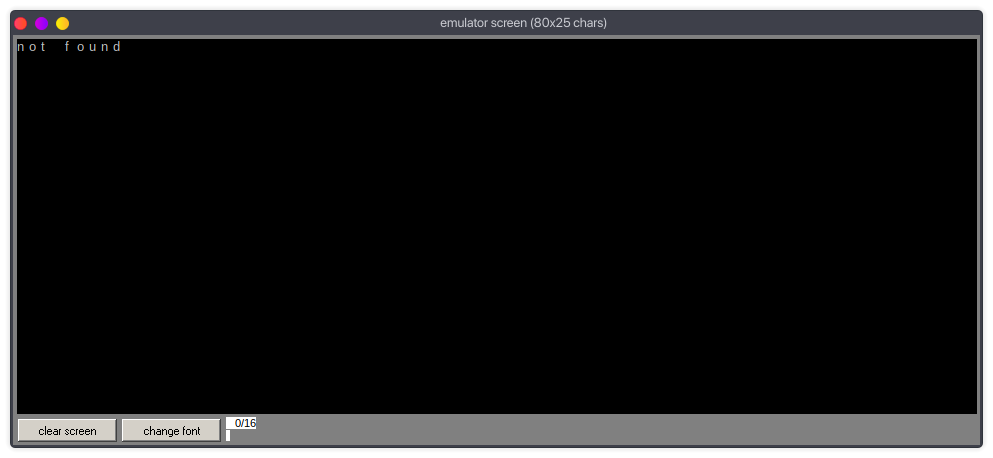
\includegraphics[width=0.90\textwidth]{img/p19/ss5.png} \\
	Output for 'lx'
\end{center}

\subsection{Result}
A substring was checked to be present in a string

